\subsubsection{Analysis}
The gate driver selected for this design is the SI8261BAC-C-IS\cite{Si8261} from Silicon Labs. It is driven by the $3.3V$ output of the Zybo while providing an output of $12V$, constrained by the attached $12V$ floating supply Cosel MGS1R54812\cite{MGS1R5}. A floating supply is required for the high-side to be able to take on a potential independent of the power ground when its drain and source potential is constrained by the load and the battery voltage. The gate driver's ground floats along with the source potential of the FET so it is always able to provide a voltage of $12V$ between the gate and the source. The advantage of having an isolated supply for the low-side as well is better noise tolerance - the FETs reference level is made somewhat independent of the ripple current on the power ground from all the loads. The high-side floating supply also has the advantage over a bootstrap capacitor of not requiring  part of an output cycle to be used for charging the capacitor. This way more power can be used to propel the gokart.

\begin{figure}[H]
	\centering
	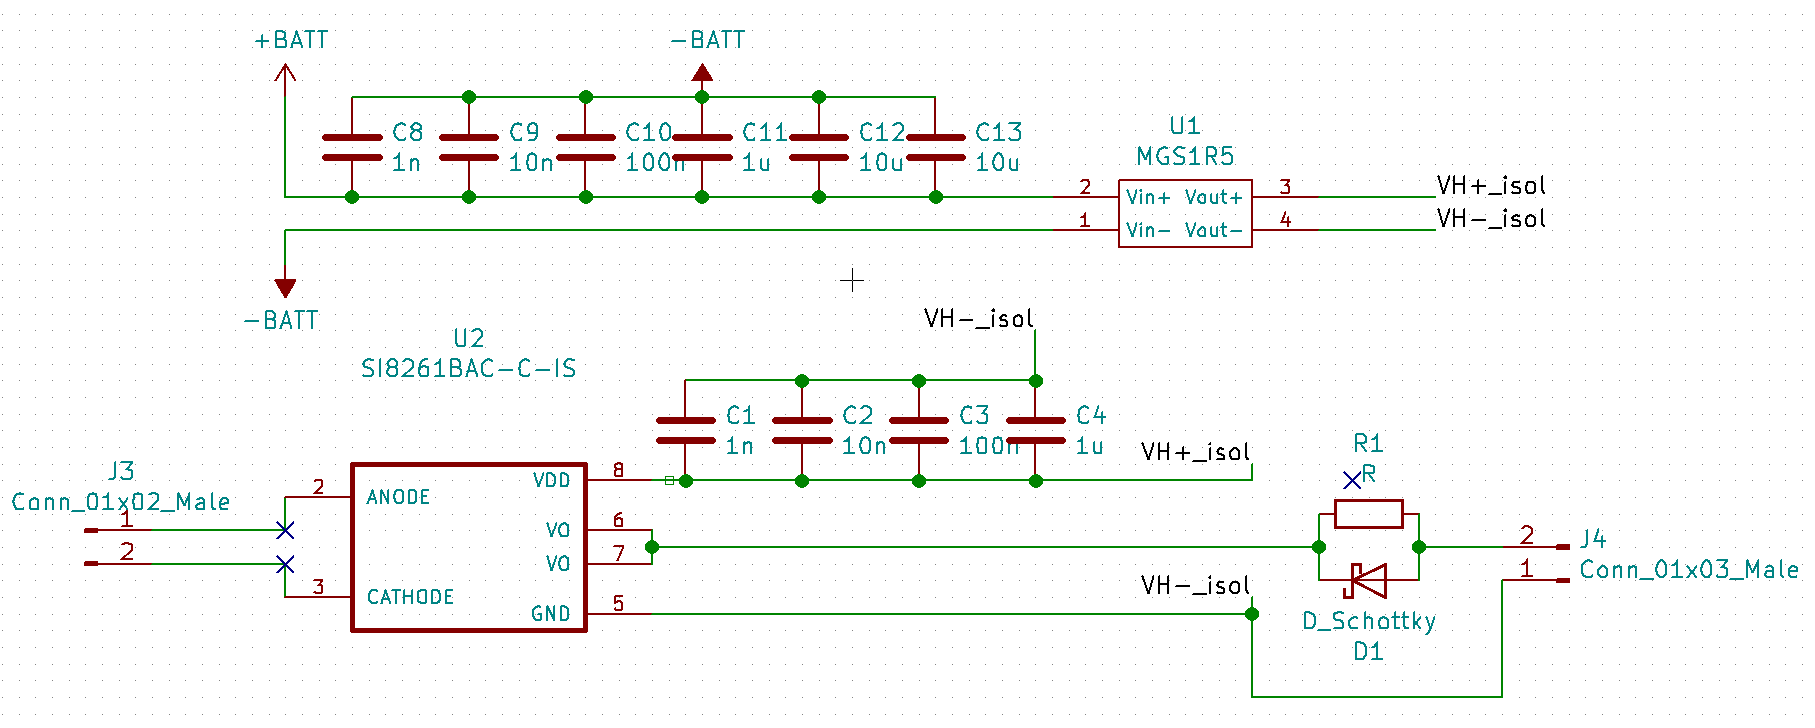
\includegraphics[width=0.6\linewidth]{pictures/hardware/Driver_Board/driver_circuit.png}
	\caption{One leg of one phase of the driver circuit}
	\label{fig:driver_circuit}
\end{figure}

 Figure \ref{fig:driver_circuit} shows the driver of one leg of one phase. Separate drivers were chosen for the separate legs of each phase to reduce the thermal stress of the individual IC-s. The low-side and the high-side driver circuit is identical. \\

A series of capacitors is attached both to the input and output of the floating supply. The smaller ones are meant to serve as high-frequency decouplers while the $10$$\mu$$F$  ones are the bulk capacitors to prevent droop on the $12V_{DC}$ rail. This helps with countering the noise-emitting effects of the long wires and quick transients from the battery when load changes rapidly. \\

The turnon and turnoff times were chosen to be around the slower end of the available range to make the circuit less prone to overshoot and ringing caused by the parasitic inductances and capacitances inherently present in the layout. The analysis of deciding the switching frequency is detailed in section \ref{switching_frequency}. \\

In Figure \ref{fig:CSI_current} and Figure \ref{fig:skew_current} taken from TIDA-00364\cite{TIDA-00364} reference design by TI, the use of split gate resistors can be seen. These consist of R2, which is common to all the parallel MOSFETs, and R20 through 24, which are individual to each MOSFET . R2 helps to easily change the turnon gate current of all the parallel FETs by changing a single resistor instead of changing each of the individual resistors. R20 through R24 help in suppressing the circulating current between the gate of the MOSFETs, which may cause gate voltage ringing. To describe the mechanism, consider only two FETs in parallel as shown in Figure \ref{fig:CSI_current} . Due to the layout, the parasitic common source inductance (CSI) of all the FETs will not be equal. If both the FETs are turned on the same instant and if the di/dt of the drain currents are equal, the voltage across CSI of both FETs (VLs1 and VLs2) will not be equal. This drives a circulating current as shown in Figure \ref{fig:skew_current} . Another possibility is if there is a skew in the $V_{DS}$ rise and fall time of the parallel FETs, circulating current can flow through the $C_{GD}$ as shown in Figure \ref{fig:skew_current} and cause unwanted behavior. Using individual gate resistors help to suppress the circulating current and help damp unwanted ringing effects. Due to a misunderstanding, we failed to place split resistors, only one is placed at the output of the driver IC, parallel to a diode meant to provide quicker turn-off times. In the upcoming sections the case of the split resistors will be further examined, as it was the original plan.

\begin{figure}[H]
	\centering
	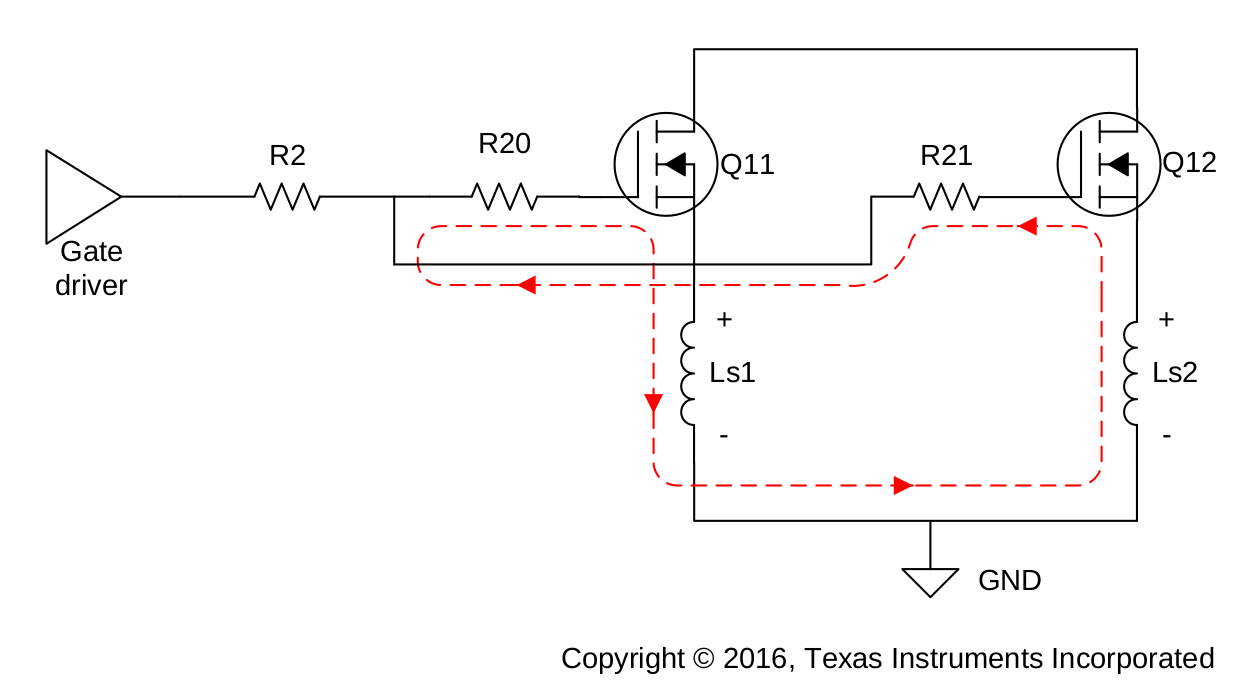
\includegraphics[width=0.6\linewidth]{pictures/hardware/Driver_Board/CSI.png}
	\caption{Gate circulating current due to CSI}
	\label{fig:CSI_current}
\end{figure}

\begin{figure}[H]
	\centering
	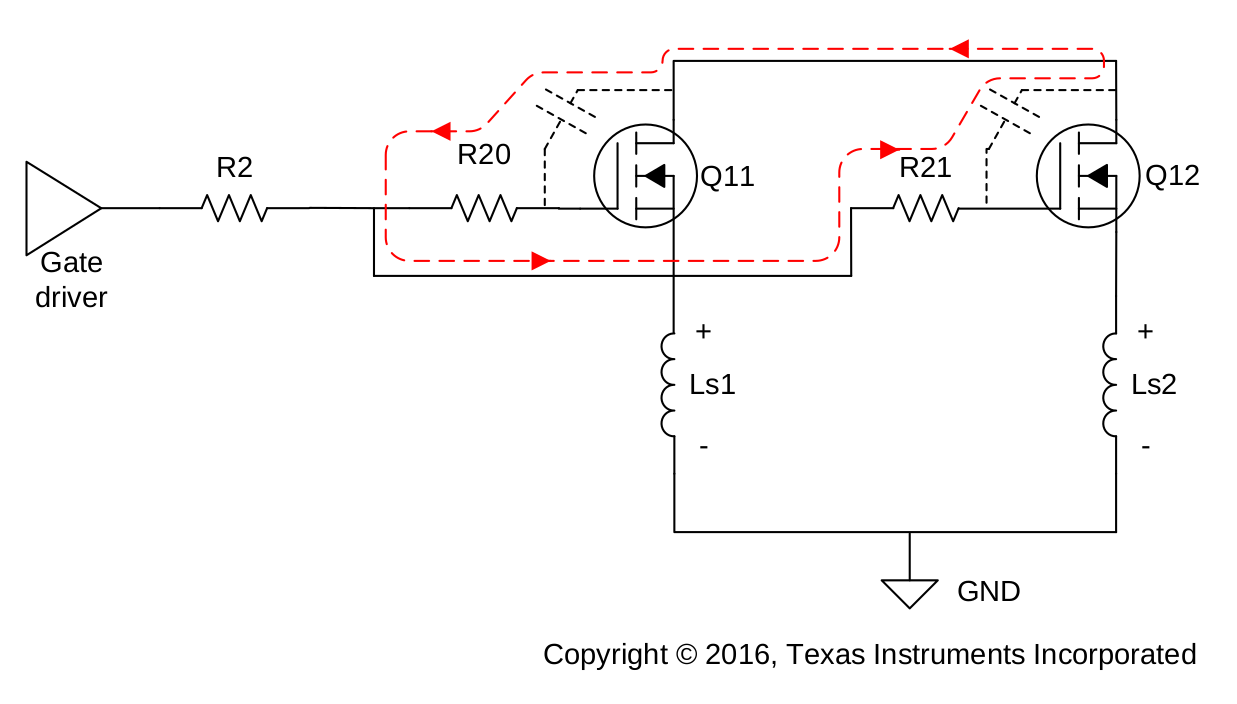
\includegraphics[width=0.6\linewidth]{pictures/hardware/Driver_Board/skew.png}
	\caption{Gate circulating current due to skew}
	\label{fig:skew_current}
\end{figure}